\documentclass[11pt]{article}
\usepackage{geometry}                % See geometry.pdf to learn the layout options. There are lots.
\geometry{letterpaper}                   % ... or a4paper or a5paper or ... 
%\geometry{landscape}                % Activate for for rotated page geometry
\usepackage[parfill]{parskip}    % Activate to begin paragraphs with an empty line rather than an indent
\usepackage{graphicx}
\usepackage{amssymb}
\usepackage{epstopdf}
\usepackage{hyperref}
\usepackage{float}
 \usepackage{color}
 \usepackage{graphicx}
\usepackage[space]{grffile}

\DeclareGraphicsRule{.tif}{png}{.png}{`convert #1 `dirname #1`/`basename #1 .tif`.png}

\title{{ISSE User Manual} \\ \vspace{0cm} \url{isse.sourceforge.net} \\ \vspace{13cm}}
\author{Version 0.2.0 (alpha) \\ The ISSE Team }
\date{\today}                                           % Activate to display a given date or no date




\begin{document}
\maketitle

\newpage

%%%%%%%%%%%%%%%%%%%%%%%%%%%%%%%%%%%%%%%%%%%%%%%%%%%%%%%%%%%%%%%%%%%%%%%%%%%%%%%%
\section*{Preface}
For an updated manual, please always see \textcolor{blue}{\url{http://isse.sourceforge.net/Manual.pdf}}.



%%%%%%%%%%%%%%%%%%%%%%%%%%%%%%%%%%%%%%%%%%%%%%%%%%%%%%%%%%%%%%%%%%%%%%%%%%%%%%%%
\section{About}
ISSE is an interactive sound source separation editor.  It allows you to  import a single audio recording and separate it into two distinct sound sources via drawing and painting tools.  Example tasks include separating a cell  phone ring from recorded speech, separating drums mixed with bass guitar,  or separating vocals from background music. See our demo \textcolor{blue}{\href{http://isse.sourceforge.net/index.html}{video}} for more  information.

The software is an open source, freely available, cross platform audio editing tool developed by the Center for Computer Research in Music and Acoustics (CCRMA), Stanford University and Adobe Research. It is licensed under the GNU General Public License, Version 3. Authors include: \textcolor{blue}{\href{http://ccrma.stanford.edu/~njb}{Nicholas J. Bryan}}, \textcolor{blue}{\href{http://ccrma.stanford.edu/~gautham}{Gautham J. Mysore}}, and  \textcolor{blue}{\href{http://ccrma.stanford.edu/~ge}{Ge Wang}}.

For questions or comments, please see our
\begin{itemize}
\item Main web site  \textcolor{blue}{\url{http://isse.sourceforge.net/}}
\item User forum  \textcolor{blue}{\url{http://isse.sourceforge.net/forum/}}
\item Wiki  \textcolor{blue}{\url{http://isse.sourceforge.net/wiki}}
\item Mailing list  \textcolor{blue}{\url{http://isse.sourceforge.net/contact.html}}.
\end{itemize}


%%%%%%%%%%%%%%%%%%%%%%%%%%%%%%%%%%%%%%%%%%%%%%%%%%%%%%%%%%%%%%%%%%%%%%%%%%%%%%%%
\section{Installation}

%%%%%%%%%%%%%%%%%%%%%%%%%%%%%%%%%%%%%%%%%%%%%%%%%%%%%%%%%%%%%%%%%%%%%%%%%%%%%%%%
\subsection{OSX}
\begin{enumerate}
\item Download the latest version at  \textcolor{blue}{\href{http://isse.sourceforge.net/download.html}{isse.sourceforge.net/download.html}}
\item Double-click the ISSE.dmg file. This will open the ISSE disk image.
\item Click-and-drag the ISSE application into your Applications folder.
\item (Optional) Copy the additional materials (test files, manual, etc.).
\item Done!  
\end{enumerate}

%%%%%%%%%%%%%%%%%%%%%%%%%%%%%%%%%%%%%%%%%%%%%%%%%%%%%%%%%%%%%%%%%%%%%%%%%%%%%%%%
\subsection{Windows}
\begin{enumerate}
\item Download the latest version at  \textcolor{blue}{\href{http://isse.sourceforge.net/download.html}{isse.sourceforge.net/download.html}}
\item Double-click the ISSE-Setup.exe file. This will open the ISSE installer.
\item Following the installation steps.
\item Note, additional materials (test files, manual, etc.) are also installed along with the application.
\item Done!  
\end{enumerate}

%%%%%%%%%%%%%%%%%%%%%%%%%%%%%%%%%%%%%%%%%%%%%%%%%%%%%%%%%%%%%%%%%%%%%%%%%%%%%%%%
\subsection{Linux}
\begin{enumerate}
\item Download the latest version of the code at  \textcolor{blue}{\href{http://sourceforge.net/p/isse/code/ci/master/tree/}{sourceforge.net/p/isse/code/ci/master/tree/}}
\item Following the compilation steps from at \textcolor{blue}{\href{http://isse.sourceforge.net/wiki/index.php/Developer}{isse.sourceforge.net/wiki/index.php/Developer}}.
\item Compile as needed per platform....
\item Done! 
\item Note: we will eventually support installation packages, but at this time only the source code (tested on Fedora) is available.
\end{enumerate}

%%%%%%%%%%%%%%%%%%%%%%%%%%%%%%%%%%%%%%%%%%%%%%%%%%%%%%%%%%%%%%%%%%%%%%%%%%%%%%%%
\section{Quick Start}

\begin{enumerate}
\item For a quick introduction to the application, please see the demo video posted at \newline  \textcolor{blue}{\url{http://isse.sourceforge.net/index.html}}. 
\item Open the application and start a new project via: File $\rightarrow$ New. 
\item Select a short (5-30 second) .wav file.  Longer files are permitted, but will be slow to process.  If needed, select  one of the example files from the \emph{Test Files} folder of the download package.
\item View and listen to the sound.  Time goes from left to right. Frequency goes from bottom to top. You can zoom, scroll, etc. Click the play button at the top or hit spacebar to listen.
\item Choose which sound you would like to separate (e.g. vocals vs. background music, cell phone ring vs. speech, etc.).
\item Associate one of the two colors from the top left to a given sound (e.g. vocals).  Associate the remaining color for the remaining sound in the recording (e.g. background music).
\item Start annotating the visualization of sound.  Select one of the drawing/painting tools (e.g. brush, time select, frequency select, box select).
Draw on salient regions of the visualization that correspond to each sound source (e.g. drums, bass, vocals, etc).  Use the brush controls (click the plus sign to right of the brush tools) as a measure of confidence. You do not have to annotate the entire file. 
\item Click the process button (upper right). Wait a little bit and the middle and bottom audio tracks will soon display the separated results. When the processing button is on the results will continually update in the background.
\item Listen and view the separated results. They won't be perfect, but...!
\item Repeat the annotation process.   Now draw on the input and output to refine the separation. 
\item Export the separated results via:  File $\rightarrow$ Export Audio and save the project via:  File $\rightarrow$ Save As.  Note, to save, export audio, open, and create new projects, the processing button must be off and the processing progress bar must 100\%.
\item Done!
\end{enumerate}
\begin{figure}[h!]
\centering
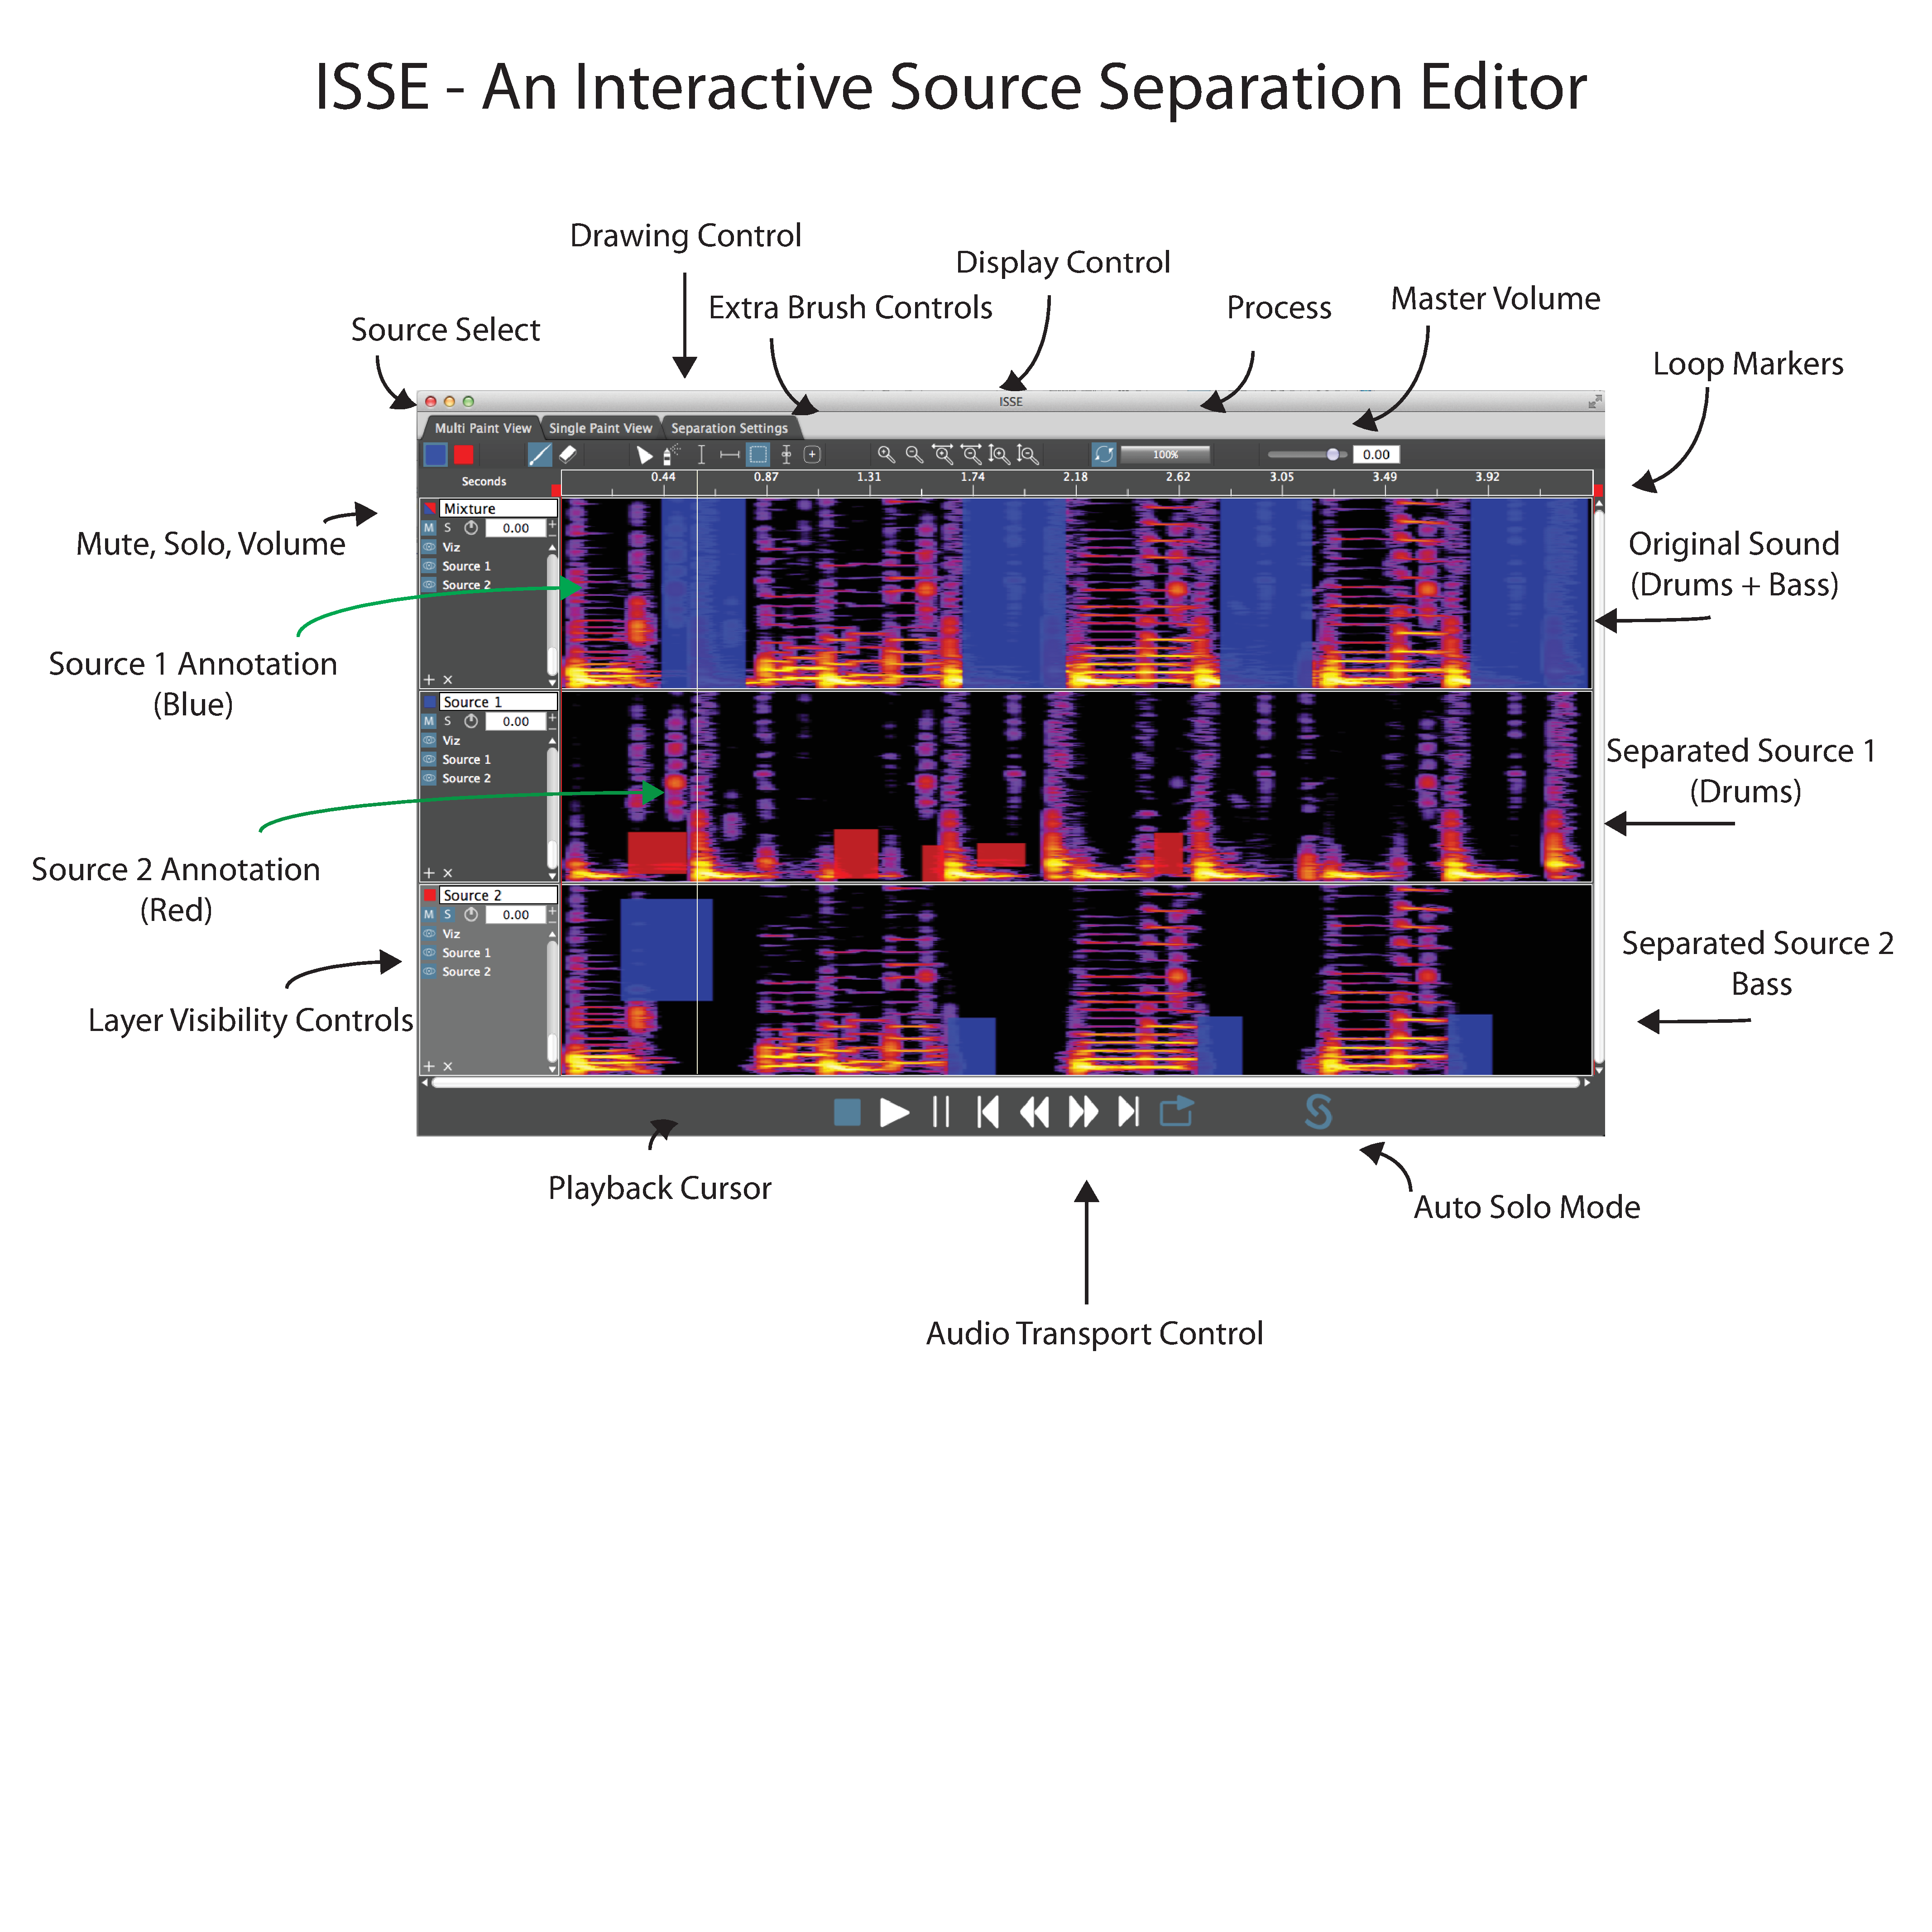
\includegraphics[trim = 2cm 0mm 0mm 0mm, width=1.1\textwidth]{images/ISSE-Quick-Start.pdf}
\caption{Quick Start Guide to ISSE.}
\label{fig:ise}
\end{figure}



\newpage
\section{Screenshots}
To give a better idea of some of the functionality of ISSE, please see the screenshots below.

\begin{figure}[h!]
\centering
\includegraphics[trim = 2cm 0mm 0mm 0mm, width=1.\textwidth]{{images/Multi Paint View.png}}
\caption{The Multi Paint View. In this view, you can see both the input audio file and the two outputs.}
\end{figure}
\begin{figure}[h!]
\centering
\includegraphics[trim = 2cm 0mm 0mm 0mm, width=1.\textwidth]{{images/Single Paint View.png}}
\caption{The Single Paint View. In this view, you get a larger screen space to view a single track.}
\end{figure}
\begin{figure}[h!]
\centering
\includegraphics[trim = 2cm 0mm 0mm 0mm, width=1.\textwidth]{{images/Settings View.png}}
\caption{The Separation Settings View. In this view, you change parameters of the separation algorithm. Careful, changing certain settings can clear your painting annotations (an alert box will tell you which ones...).  }
\end{figure}
\begin{figure}[h!]
\centering
\includegraphics[trim = 2cm 0mm 0mm 0mm, width=1.\textwidth]{{images/Visualization Settings.png}}
\caption{The Visualization Settings View. In this view, you change parameters that control the visualization of sound such as the color map and the clip limit. }
\end{figure}
\begin{figure}[h!]
\centering
\includegraphics[trim = 2cm 0mm 0mm 0mm, width=1.\textwidth]{{images/Brush Settings.png}}
\caption{The Brush Settings View. In this view, you change additional painting brush parameters. Click the plus sign to the right of the brush icons. }
\end{figure}
\begin{figure}[h!]
\centering
\includegraphics[trim = 2cm 0mm 0mm 0mm, width=1.\textwidth]{{images/Audio Settings.png}}
\caption{The Audio Settings View. In this view, you can change the audio settings (sample rate, buffer size, etc.). To open this view, go to File $\rightarrow$ Audio Settings. }
\end{figure}


\section{Technical Documentation} 
Technical publication on the source separation algorithm use within ISSE can be found at:
\begin{itemize}
\item \cite{Bryan2013A} - An extended abstract and introduction to the idea.
\item \cite{Bryan2013B} - The core algorithm and technical material.
\item \cite{Bryan2013C} - Algorithmic extensions and additional interpretation.
\end{itemize}

\bibliographystyle{unsrt}
\bibliography{references}

\end{document}  









